\documentclass[parskip=half,a4paper,portrait]{scrartcl}

\input{../../../structure.tex}

\usepackage{float}

\title{Machine Learning Exercise 4}
\author{Laszlo Korte, MtrNr. 6329857}
\date{Universität Hamburg --- \today}




\begin{document}

\maketitle

\begin{figure}[H]
\begin{center}
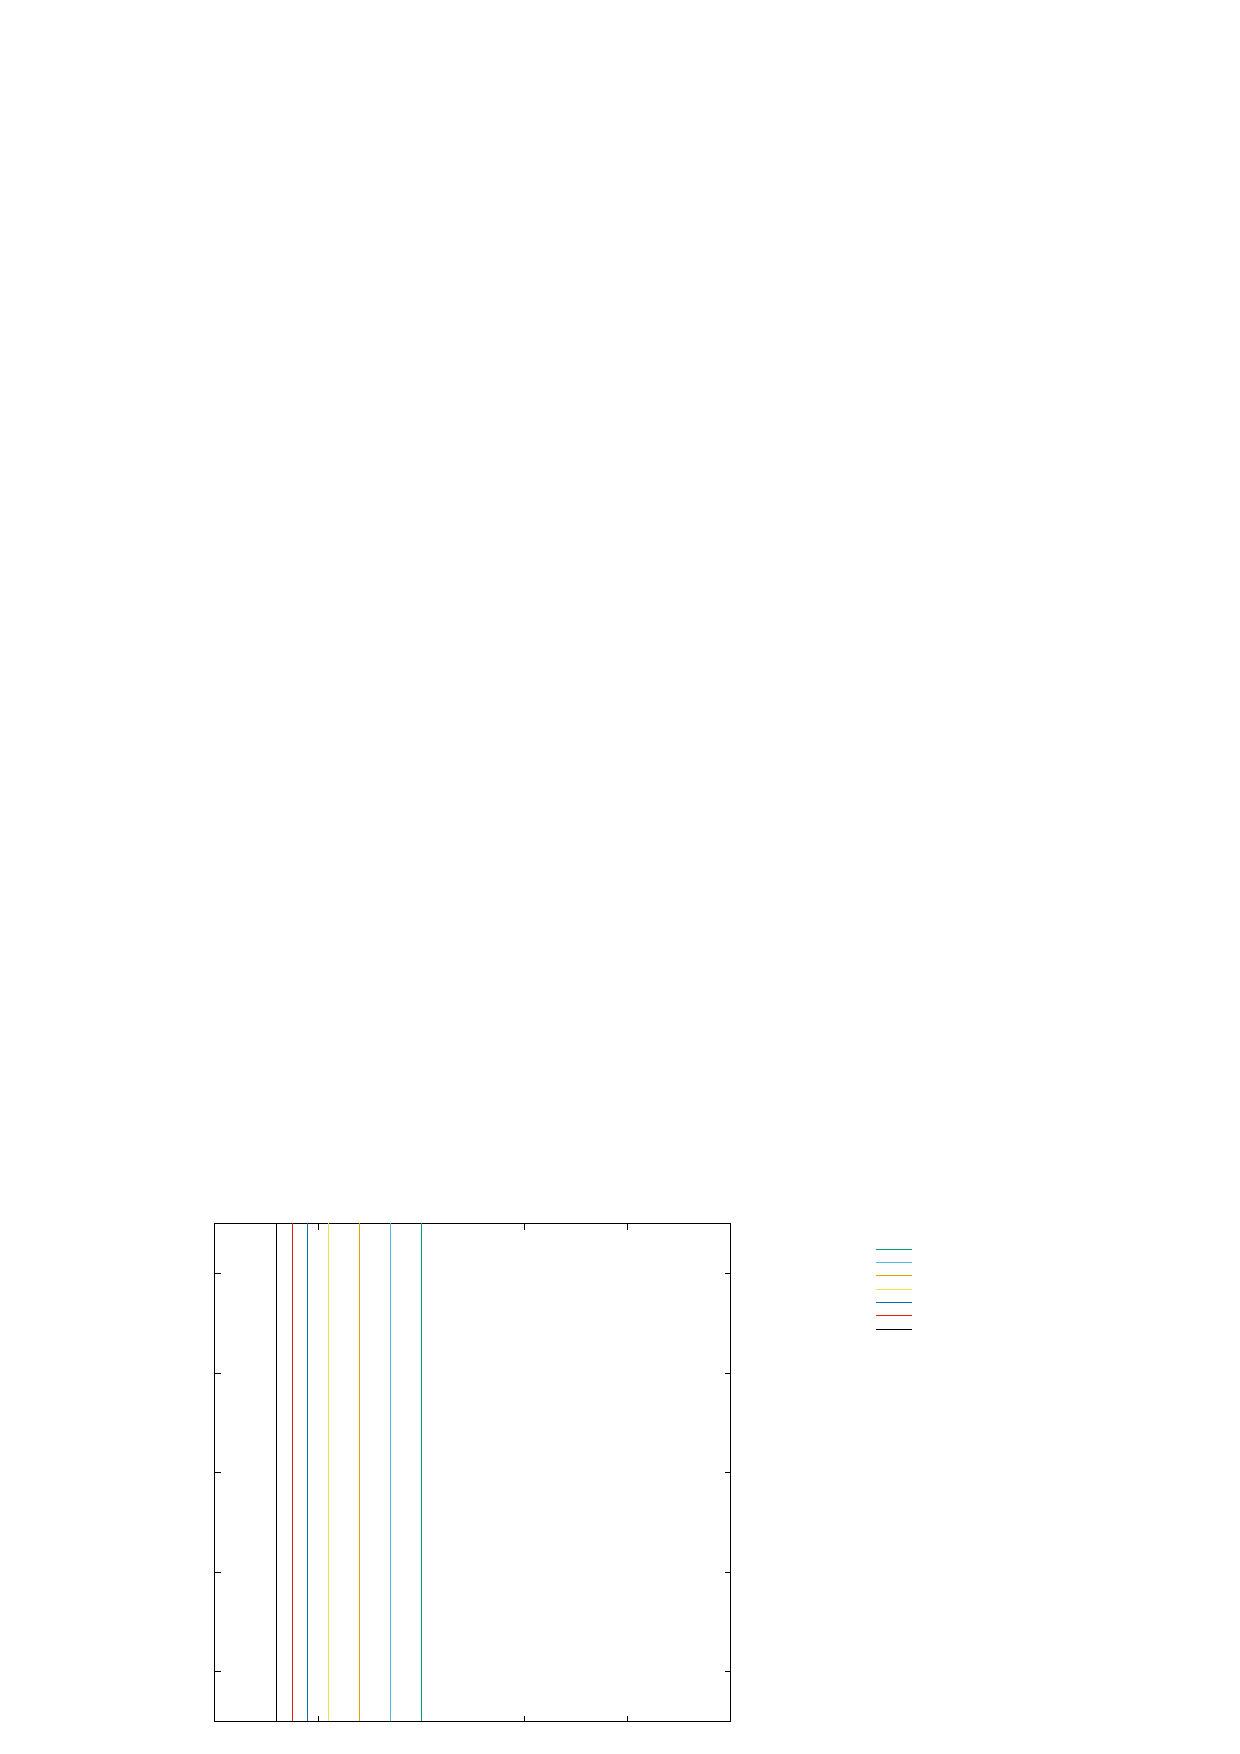
\includegraphics[trim={3cm 2cm 0 4cm},clip]{var/grid-linear.pdf}
\caption[Grid search with linear kernel]{Linear Kernel\\Best $\log_2(C) = -8.0$,
$\log_2(\gamma) = 0.0$,
$\text{accuracy} = 100.0\%$,
$C = 0.00390625$, $\gamma = 1.0$}
\end{center}
\end{figure}

\begin{figure}[H]
\begin{center}
\includegraphics[trim={3cm 1cm 0 4cm},clip]{var/grid-polynomial.pdf}
\caption[Grid search with polynomial kernel]{polynomial Kernel\\Best $\log_2(C) = -10.0$, $\log_2(\gamma) = -3.0$, $\text{accuracy} = 100.0\%$, $C = 0.0009765625$, $\gamma = 0.125$}
\end{center}
\end{figure}

\begin{figure}[H]
\begin{center}
\includegraphics[trim={3cm 1cm 0 4cm},clip]{var/grid-radial.pdf}
\caption[Grid search with Radial kernel]{Radial Kernel\\Best $\log_2(C) = -8.0$, $\log_2(\gamma) = 0.0$, $\text{accuracy} = 100.0\%$, $C = 0.00390625$, $\gamma = 1.0$}
\end{center}
\end{figure}

\begin{figure}[H]
\begin{center}
\includegraphics[trim={3cm 1cm 0 4cm},clip]{var/grid-sigmoidal.pdf}
\caption[Grid search with Sigmoidal kernel]{Sigmoidal Kernel\\Best $\log_2(C) = 2.0$, $\log_2(\gamma) = -10.0$, $\text{accuracy} = 100.0\%$, $C = 4.0$, $\gamma = 0.0009765625$}
\end{center}
\end{figure}



\end{document}

